\begin{sol}
\begin{enumerate}[label=\textbf{(\alph*)}] 
\item Let us first draw a diagram. 
\begin{center}
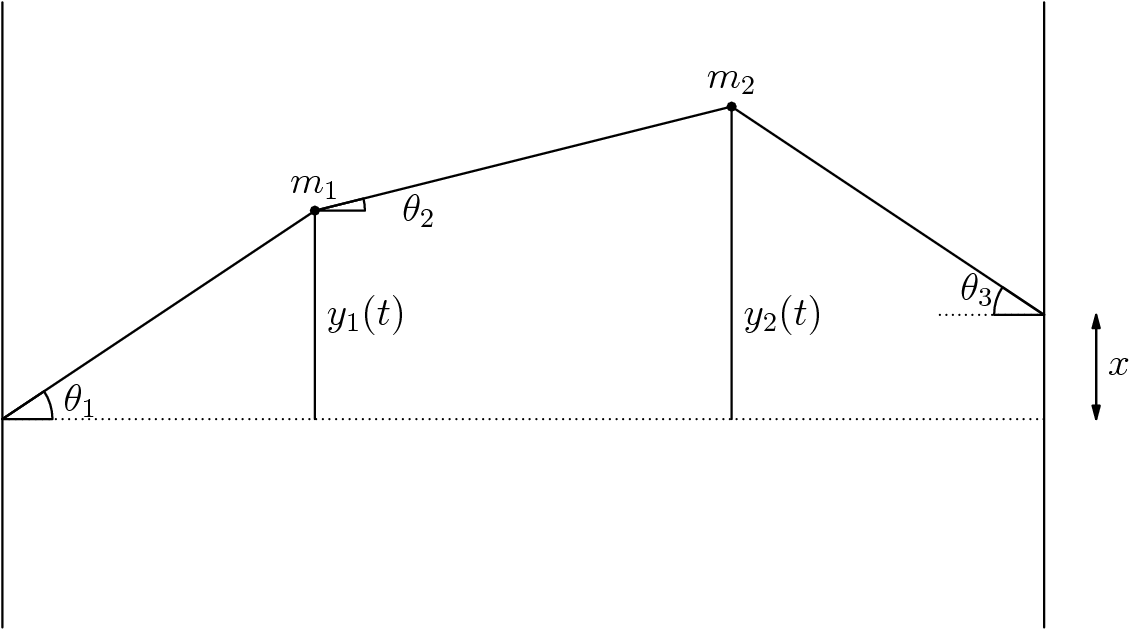
\includegraphics[width=\linewidth]{P03/ropes2.png}
\end{center}
\end{enumerate}
Since the angles are small, and the horizontal components of tension are approximately the same and can be approximated by 
\[T_1\cos\theta_1 \approx T_2\cos\theta_2 \approx T_3\cos\theta_3\implies T_1 \approx T_2 \approx T_3 = T.\]
We can approximate the sines of the angles by 
\begin{align*}
    \sin\theta_1 &= \frac{y_1(t)}{a} \\
    \sin\theta_2 &= \frac{y_2(t) - y_1(t)}{a} \\
    \sin\theta_3 &= \frac{y_2(t)}{a}
\end{align*}
where $a$ is the length of each component of the rope. For $m_1$, we have 
\[m_1 \ddot{y}_1 = T_2\sin\theta_2 - T_1\sin\theta_1\]
and using our approximations tells us that 
\[\boxed{\ddot{y}_1 = \frac{T}{m_1 a} (y_2 - 2y_1)}.\]
Similarly, we have for $m_2$, 
\[\boxed{\ddot{y}_2 = \frac{T}{m_2 a}(y_1 - 2y_2)}.\]

\item 
\end{sol}